\section{Common part}
\subsection{Anti-aliasing}
In computer graphics using raster images can lead to "stairstepping" or aliasing. Aliasing can generally be replaced by noise, if the ray origins are randomly placed inside a pixel. Fully random placement of the ray-starting point is not optimal, as the randomly distributed pixels can clump together and leave some areas poorly sampled. Therefore each pixel is subdivided into sub-areas and each sub-area is given one sample. This is called jittered sampling. 


\subsection{Area Lights}
In contrast to point lights, area lights have a surface. In order to solve the rendering equation for scenes lit by area lights, the area form of the rendering equation is considered \footnote{Ray Tracing from the ground up page 329}:
\begin{equation}
\mathbf{L}_r(\mathbf{p},\mathbf{\omega}_0) = \int_{A_{light}} f_r(\mathbf{p},\mathbf{\omega}_i,\mathbf{\omega}_0) \mathbf{L}_e(\mathbf{p}',-\mathbf{\omega}_i)V(\mathbf{p},\mathbf{p}')G(\mathbf{p},\mathbf{p}')dA_{\mathbf{p}'}
\end{equation}
The above equation allows it to find the outgoing light at a primary ray intersection point $\mathbf{p}$. Given the reflection orientation vector $\mathbf{\omega}_0$ and the incoming light direction $\mathbf{\omega}_i = (\mathbf{p} - \mathbf{p}') / \|\mathbf{p} - \mathbf{p}'\|$. The visibility function $V(\mathbf{p}',\mathbf{p})$ is one if point $\mathbf{p}$ is visible from point $\mathbf{p}'$ and zero if not. The geometry term $G$ is given by:
\begin{equation}
G = \frac{cos (\theta_i) cos (\theta')}{\| \mathbf{p}' - \mathbf{p}\| ^ 2}
\end{equation}  
With $cos (\theta_i), cos (\theta')$ given by $\mathbf{n}_\mathbf{p} ^ T \mathbf{\omega}_i$ and $\mathbf{n}^{T}_{\mathbf{p}'} (-\mathbf{\omega}_i)$ respectively. Finally $\mathbf{p}'$ must be a random point within the area light source.
The solution of the rendering equation can be estimated by using Monte-Carlo integration:
\begin{equation}
\mathbf{L}_r(\mathbf{p},\mathbf{\omega}_0) \approx \frac{1}{n_s} \sum_{j=1}^{n_s} \frac{f_r(\mathbf{p},\mathbf{\omega}_{i,j},\mathbf{\omega}_0) \mathbf{L}_e(\mathbf{p}',-\mathbf{\omega}_{i,j})V(\mathbf{p},\mathbf{p}_j')G(\mathbf{p},\mathbf{p_j}')}{p(\mathbf{p}')}
\end{equation}
Here $n_s$ denotes the number of samples, and $p(\mathbf{p}')$ the probability density function. The simplest choice is to distribute the samples uniformly which leads to $p(\mathbf{p}') = \frac{1}{A_l}$. A scene with a spherical and planar light source is shown in figure~\ref{fig:borgEarth}. Using area light sources leads to smooth shadows, like to those caused by the cubes on the earth's surface. 


\begin{figure}
\centering
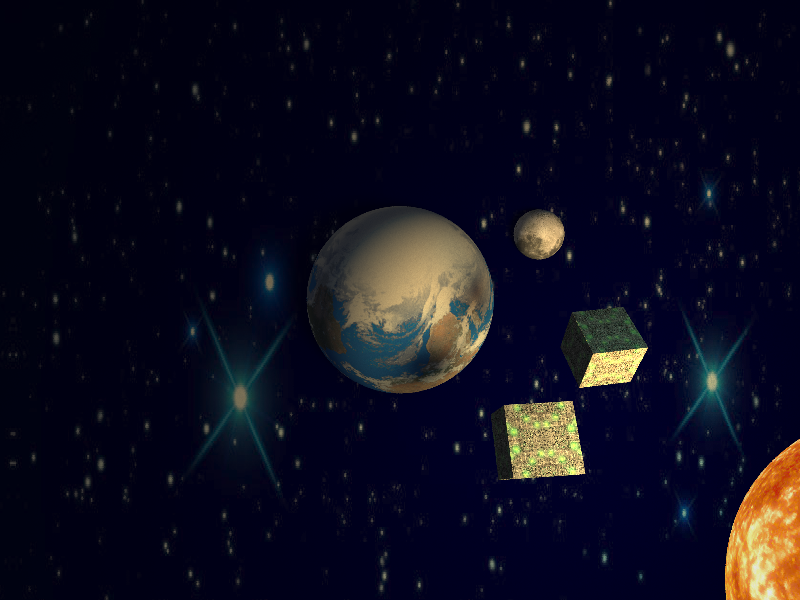
\includegraphics[width=0.5\linewidth]{./img/borgEarth3}
\caption{A spherical area light causing smooth shadows on a sphere}
\label{fig:borgEarth}
\end{figure}
\begin{figure}
\centering
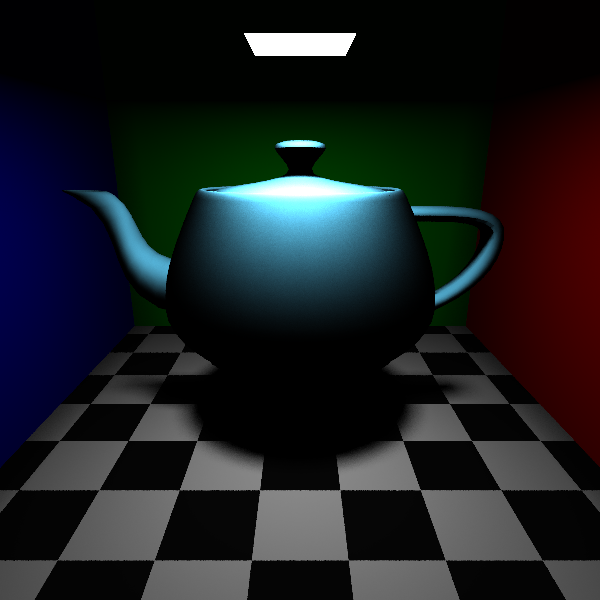
\includegraphics[width=0.5\linewidth]{./img/areaTeapot}
\caption{A rectangular area light illuminating the Utah teapot}
\label{fig:areaTeapot}
\end{figure}


\section{Special effects}
\subsection{Normal Mapping}
In order to add additional normal information or speed up the rendering of wavefront objects, normal data can be loaded from a file. The normal-information is coded as:
\begin{align*}
c_r = 0.5 + 0.5 \cdot n_x \\
c_g = 0.5 + 0.5 \cdot n_y \\
c_b = 0.5 + 0.5 \cdot n_z
\end{align*}
which can be transformed back using:
\begin{align}
n_x = -1.0 + 2*(c_r/255) \\
n_y = -1.0 + 2*(c_g/255) \\
n_z = -1.0 + 2*(c_b/255)
\end{align}
The normal information can then be used for rendering purposes. In case of the Stanford dragon shown in figure~\ref{fig:dragonNormlMap} it took 32s for the high resolution mesh and 6.02s for the low resolution mesh with normal map to produce the same result. 
\begin{figure}
\centering

\includegraphics[width=0.33\linewidth]{./img/dragonHighResMap}

\includegraphics[width=0.33\linewidth]{./img/dragonNormlMap}
\caption{Stanford-Dragon on plane rendered using a high resolution mesh (left) and low resolution mesh with normal map(right).}
\label{fig:dragonNormlMap}
\end{figure}


\subsection{Physical materials}
An important factor in improving the quality of the rendered images is the bidirectional reflectance distribution function (brdf) $f_r(\mathbf{p},\mathbf{\omega}_i,\mathbf{\omega}_0)$. The brdf-model may be split into a diffuse and specular component
\begin{equation}
f_r(\mathbf{p},\mathbf{\omega}_i,\mathbf{\omega}_0) = f_d(\mathbf{p},\mathbf{\omega}_i) + \rho_s f_s(\mathbf{p},\mathbf{\omega}_i,\mathbf{\omega}_0).
\end{equation}
In this project a lambertian
\begin{equation}
f_d(\mathbf{p},\mathbf{\omega}_i) = \frac{\rho_d}{\pi} cos(\theta_i)
\end{equation}
model is used for diffuse part. $\theta_i$ denotes the angle between incoming light and surface normal. The cosine term can be computed using $\mathbf{n}_{\mathbf{p}}^T \mathbf{\omega}_i = cos(\theta_i)$.  
For the specular part a Phong reflection model 
\begin{equation}
f_s(\mathbf{p},\mathbf{\omega}_i,\mathbf{\omega}_0) = \rho_s (\mathbf{r}^T \mathbf{\omega}_0)^e
\end{equation}
is considered.\footnote{Ray Tracing from the ground up page 281} The vector $r$ denotes the mirror reflection direction.  Furthermore a Cook-Torrance model for the specular part has been implemented. This model is taken from their original 1982 publication: \footnote{A Reflectance Model for Computer Graphics, Robert L. Cook, Kenneth E. Torrance, ACM Transactions on Graphics, Vol. 1, No. 1, January 1982, Pages 7-24}
\begin{align}
\mathbf{h} &= \frac{\mathbf{c} + \mathbf{\omega}_i}{\| \mathbf{c} + \mathbf{\omega}_i \|} \\
c & = \mathbf{c}^T \mathbf{h} \\
g &=  \sqrt{n*n + c*c - 1} \\
n &= \frac{1 + \sqrt{f_0}}{1 - \sqrt{f_0}} \\
F &= \frac{1}{2} \frac{(g - c)^2}{(g + c)^2} (1 + \frac{[c (g + c) - 1]^2}{[c (g - c) + 1]^2}) \\
\alpha &= \cos^{-1}(\mathbf{h}^T \mathbf{n}_\mathbf{p}) \\
D &= \frac{1}{m^2 cos^4(\alpha)}e^{[-(\tan(\alpha)/m)]^2} \\
G &= \min(1,
     \frac{2 (\mathbf{n}_\mathbf{p}^T \mathbf{h})(\mathbf{n}_\mathbf{p}^T \mathbf{c})  }{(\mathbf{c}^T \mathbf{h})}),
     \frac{2 (\mathbf{n}_\mathbf{p}^T \mathbf{h})(\mathbf{n}_\mathbf{p}^T \mathbf{\omega}_i)  }{(\mathbf{c}^T \mathbf{h})}) \\
f_s(\mathbf{p},\mathbf{\omega}_i,\mathbf{c}) &= \frac{\rho_s}{\pi}
 \frac{DG}{(\mathbf{n}_{\mathbf{p}}^T \mathbf{\omega}_i)(\mathbf{n}_{\mathbf{p}}^T \mathbf{c})} F(c,g) \\
\end{align} 
The model depends on the two input parameters $f_0$ and $m$ as well as the scaling factor $\rho_s$. The first input is the value of the Fresnel-equation at normal incidence. The second is the root mean square slope $m$ of assumed material facets. The smaller both parameters become the less mirror like will the resulting material will be. The vectors $\mathbf{c,\omega_i}$ point to the camera and the light source respectively.
The vector $\mathbf{h}$ represents the normalized vector in the direction of the angular bisector of the view and light orientation vectors.
The $c$ variable stands for the cosine of the angle between $\mathbf{c}$ and $\mathbf{h}$ or $\omega_i$ and $\mathbf{h}$. 
The Fresnel term $F$ determines how light is reflected from each of the assumed smooth micro-facets. 
A facet slope distribution function $D$ is used. This term depends on the angle between $\mathpf{n_p}$ and $\mathbf{h}$ called $\alpha$.
Finally

\subsection{Importance Sampling}
In oder to  reduce the amount of samples required to come close to a decent approximation of the solution importance sampling is used. It's key concept is to distribute the sample points $\mathbf{p}'$ on the light source according to their contribution to the solution, important areas of the light should be sampled more often then insignificant ones. To achieve this goal the light source is subdivided into parts. A random point of each part is sampled and an importance value
\begin{equation}
I_j = i_j/I_{tot}
\end{equation}
is computed. The term $i_j$ denotes the importance value of the $j$th part of the light source, assuming that the subdivided shapes are stored in a list. The importance vlaue could for example be the product of the brdf function weighted by the geometry term of the rendering equation $i = (f_s + f_d) \cdot G$. Or if the specular part of the solution is the most important part $i = f_s$ could be used. \\
\begin{figure}
\centering
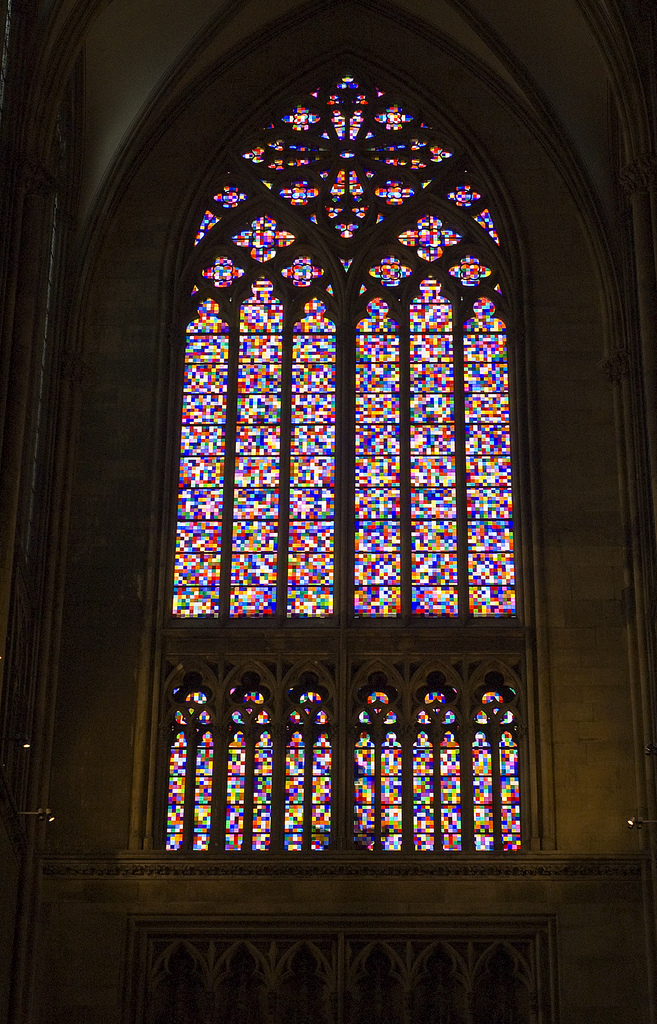
\includegraphics[width=0.25\linewidth]{./img/Richter_window_Cologne_Cathedral}
\includegraphics[width=0.25\linewidth]{./img/Kölner_Dom_Richter_Fenster}
\caption{Gerhard Richter's southern wing main window of the cologne cathedral consisting of 11.500 pixels colored using 72 different colors and pseudo-randomly arranged. On the right the lighting effect of the window on the cathedral floor can be seen.}
\label{fig:Richter_window_Cologne_Cathedral}
\end{figure}
Gerhard Richter's design of the cologne cathedral's south window and the light effects it produces is shown in figure~\ref{fig:Richter_window_Cologne_Cathedral}. Inspired by the design a rectangular light source with pseudo-randomly distributed squares has been created. This area light source is placed at a ninety degree angle on top of a floor plane. The Specular brdf-component of the floor plane will be varied. First the Phong's model is used. 
\begin{figure}
\centering
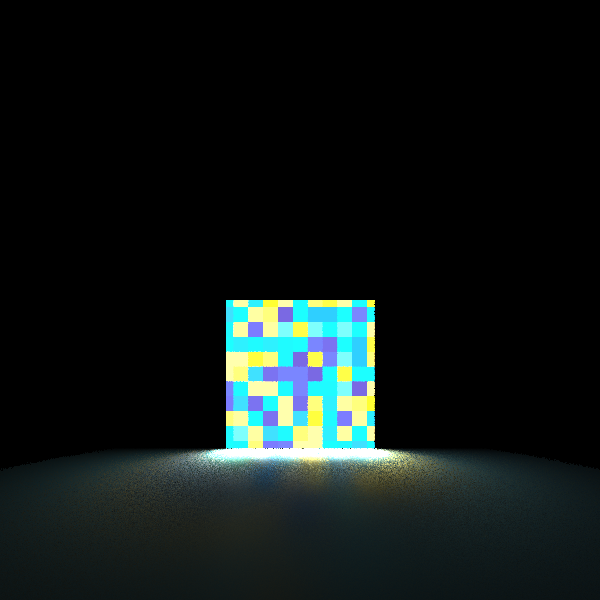
\includegraphics[width=0.3\linewidth]{./img/phong100}
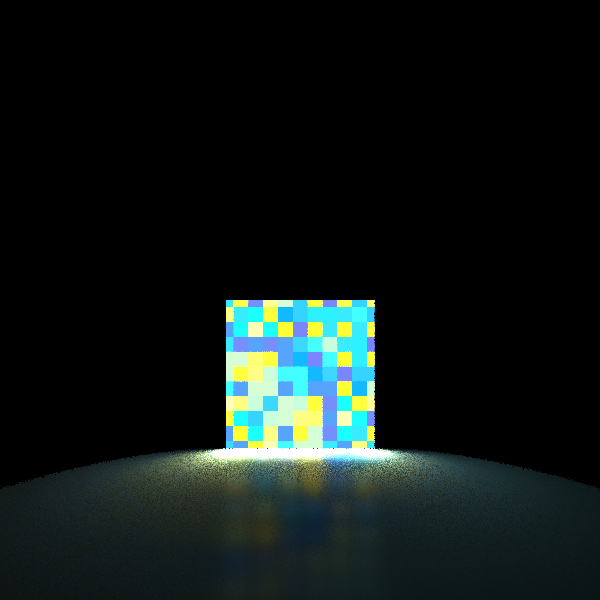
\includegraphics[width=0.3\linewidth]{./img/phong500}
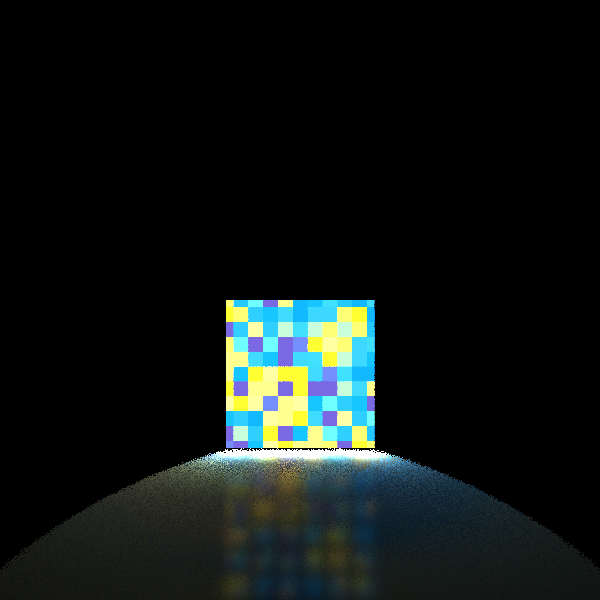
\includegraphics[width=0.3\linewidth]{./img/phong2000}
\caption{Importance sampling of Phong's specular reflection model using $e = 100$(left), $e = 500$(middle), $e = 2000$(right). In all cases $\rho_d = 0.001$ and $\rho_s = 0.999$}
\label{fig:phongRichter}
\end{figure}
Results are shown in figure~\ref{fig:phongRichter}. It can be observed that the larger the Phong-exponent $e$ is chosen, the more pronounced the reflection becomes. 
Which makes sense as with larger values for $e$ the set of possible incoming light  vectors at $\mathbf{p}$ with large specular contributions becomes smaller and smaller. Therefore the largest specular contributions come from only a small set of sample points $\mathbf{p'}$ on the light source, which are close to each other. Therefore one expects to see more detailed reflections for larger values of $e$.   \\
\begin{figure}
\centering
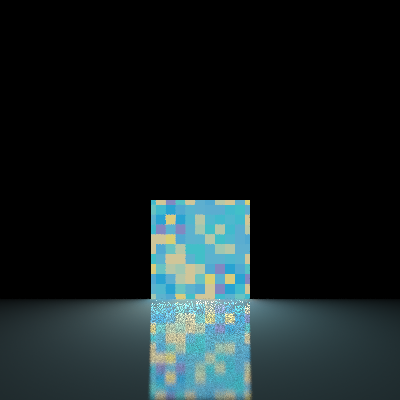
\includegraphics[width=0.3\linewidth]{./img/ct3}
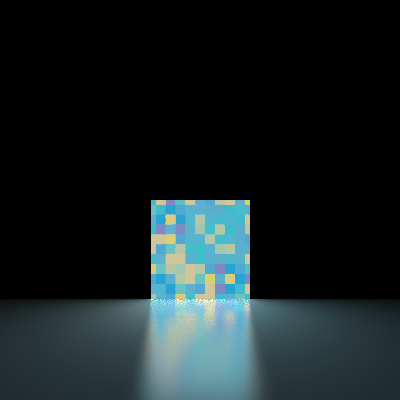
\includegraphics[width=0.3\linewidth]{./img/ct2}
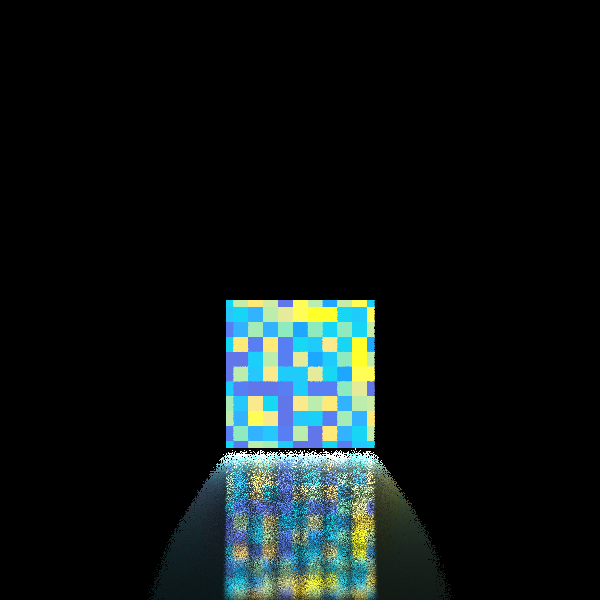
\includegraphics[width=0.3\linewidth]{./img/ct1}
\caption{Scenes computed using Cook-Torrance specular reflection models with parameters $f_0 =0.0366, m = 0.276$ (left),  $f_0 = 0.025, m = 0.076$(middle),  $f_0 = 0.03, m = 0.01$(right). In all cases $/rho_s = 1.0$ and $/rho_d = 0.5$}
\label{fig:CTRichter}
\end{figure}
In the images shown in figure~\ref*{fig:CTRichter}, the Phong model, has been replaced with a Cook-Torrance model for specular reflection. It can be observed that the larger $m$ is chosen the less visible reflection details become. Which is to be expected as $m$ models the root mean square slope of model material facets, and the larger these slopes are the more bumpy and therefore less mirror like the material will be.







